\documentclass[12pt]{article}
\usepackage[top=2.6cm,bottom=2.6cm,left=2.4cm,right=2.4cm]{geometry}
\usepackage[dvipsnames,svgnames,x11names]{xcolor}
\usepackage[T1]{fontenc}
\usepackage[utf8]{inputenc}
\usepackage[portuges]{babel}
\usepackage{amsmath,amssymb,amsfonts}
\usepackage{mathtools}
\usepackage{enumitem}
\usepackage{fancyhdr}
\usepackage{titlesec}
\usepackage{listings}
\usepackage{graphicx}
\usepackage{hyperref}
\usepackage{booktabs}
\usepackage{colortbl}
\usepackage{array}

\setlength{\parindent}{1.25em}
\setlength{\parskip}{0pt}
\pagestyle{fancy}
\fancyhf{}
\renewcommand{\headrulewidth}{0pt}
\renewcommand{\footrulewidth}{0pt}
\fancyfoot[C]{\thepage}

\titleformat{\section}{\normalfont\LARGE\bfseries}{}{0pt}{}
\titleformat{\subsection}{\normalfont\Large\bfseries}{}{0pt}{}

\lstset{
  basicstyle=\small\ttfamily,
  columns=fullflexible,
  keepspaces=true,
  showstringspaces=false,
  frame=none,
  aboveskip=0.5\baselineskip,
  belowskip=0.5\baselineskip,
  numbers=left,
  numberstyle=\small\ttfamily,
  numbersep=8pt
}

\begin{document}

\begin{titlepage}
\thispagestyle{fancy}
\vspace*{2.2cm}
\begin{center}
{\LARGE O Cavalo Perdido\par}
\vspace{1.2cm}
{\large Eduardo A. Lopes,* Nicolas Batista $\dagger$\par}
\vspace{0.15cm}
{\Large Faculdade de Informática --- PUCRS\par}
\vspace{0.8cm}
{\Large 24 de junho de 2026\par}
\end{center}

\vspace{2.1cm}

\begin{center}
{\large\bfseries Resumo}
\end{center}

Analisa-se neste trabalho o problema \emph{O Cavalo Perdido}: dado um tabuleiro $N \times N$
toroidal com casas bloqueadas, uma posição inicial \texttt{C} e uma posição de saída
\texttt{S}, determinar o menor número de movimentos que um cavalo de xadrez precisa
realizar para ir de \texttt{C} a \texttt{S}.

O tabuleiro é modelado como um grafo não-ponderado e aplica-se Busca em Largura (BFS)
para encontrar o caminho mínimo de forma ótima. A complexidade resultante é $O(N^2)$
em tempo e espaço. Os sete casos de teste fornecidos foram resolvidos com sucesso,
com tempos de execução da ordem de poucos milissegundos mesmo para tabuleiros de
$500 \times 500$.

\end{titlepage}

\setcounter{page}{2}

\section*{Introdução}

O problema estudado consiste em mover um cavalo de xadrez sobre um tabuleiro $N \times N$
com casas bloqueadas da posição inicial \texttt{C} até a posição de saída \texttt{S}
no \textbf{menor número de movimentos possível}. O cavalo move-se em ``L'': avança
2~casas em uma direção e 1~casa na direção perpendicular (ou vice-versa), gerando
8~deslocamentos possíveis.

Uma característica essencial do problema é que o tabuleiro é \emph{toroidal}: ao sair
pela borda direita o cavalo reentra pela esquerda, e o mesmo ocorre entre topo e base.
Isso torna o espaço de estados finito e sem bordas para efeito de movimento.

Uma instância pode não ter solução caso \texttt{S} seja completamente isolada por
casas bloqueadas ou esteja em uma componente desconectada de~\texttt{C}.

O enunciado fornece um exemplo com tabuleiro $20 \times 39$ (não quadrado) onde o
cavalo parte da linha~4, coluna~10 e alcança a saída na linha~14, coluna~34 em
\textbf{10~pulos}. Esse exemplo foi utilizado como caso de validação da implementação.

Nas seções a seguir apresentam-se a modelagem do problema, o algoritmo de solução,
os detalhes de implementação e a análise dos resultados.

\newpage

\section*{Modelagem do Problema}

O tabuleiro é modelado como um \textbf{grafo não-ponderado}, onde:

\begin{itemize}[leftmargin=2.2em,itemsep=0.4em]
  \item \textbf{Vértices:} cada célula $(r,c)$ que não seja bloqueada (\texttt{x})
        constitui um vértice. O grafo tem até $N^2$ vértices.
  \item \textbf{Arestas:} existe uma aresta entre $(r_1,c_1)$ e $(r_2,c_2)$ se e
        somente se o cavalo pode ir de um ao outro em um único movimento válido,
        respeitando a condição toroidal e não atingindo uma casa bloqueada no destino.
\end{itemize}

Os oito deslocamentos $(\Delta r, \Delta c)$ do cavalo são:
\[
  (\pm 1,\,\pm 2) \quad \text{e} \quad (\pm 2,\,\pm 1).
\]

No tabuleiro toroidal, a posição resultante é calculada por aritmética modular:
\[
  nr = \bigl((r + \Delta r) \bmod N + N\bigr) \bmod N,
  \qquad
  nc = \bigl((c + \Delta c) \bmod N + N\bigr) \bmod N.
\]
O termo $+N$ antes do segundo módulo garante resultado positivo quando
$r + \Delta r < 0$ (borda superior ou esquerda).

Com essa modelagem, determinar o menor número de movimentos é equivalente a encontrar
o \textbf{menor caminho entre dois vértices em um grafo não-ponderado}, problema clássico
resolvido de forma ótima pela Busca em Largura (BFS).

\vspace{0.6em}
\begin{center}
\renewcommand{\arraystretch}{1.3}
\begin{tabular}{ll}
\toprule
\textbf{Aspecto} & \textbf{Valor} \\
\midrule
Número de vértices      & $N^2$ \\
Grau máximo por vértice & 8 \\
Número de arestas       & $O(N^2)$ \\
Complexidade de tempo   & $O(V+E) = O(N^2)$ \\
Complexidade de espaço  & $O(N^2)$ \\
\bottomrule
\end{tabular}
\end{center}

\newpage

\section*{Solução}

\subsection*{Escolha do algoritmo}

A Busca em Largura (BFS) garante que a primeira vez que \texttt{S} é encontrado, o
caminho percorrido é o de \textbf{menor número de arestas} e, portanto, o menor número
de movimentos. Essa garantia é válida porque todos os movimentos do cavalo têm custo
uniforme igual a~1.

Outras alternativas foram consideradas:

\begin{itemize}[leftmargin=2.2em,itemsep=0.4em]
  \item \textbf{DFS (Busca em Profundidade):} encontra um caminho, mas não
        necessariamente o menor.
  \item \textbf{Dijkstra:} correto para grafos com pesos, porém desnecessariamente
        complexo para pesos uniformes. BFS tem complexidade $O(V+E)$, enquanto
        Dijkstra tem $O((V+E)\log V)$.
  \item \textbf{A*:} eficiente quando a heurística é boa. Para tabuleiros com
        obstáculos aleatórios e geometria toroidal, a distância euclidiana não é
        heurística admissível eficaz; e como o BFS já resolve em poucos
        milissegundos para $500 \times 500$, a complexidade extra não se justifica.
\end{itemize}

\subsection*{Algoritmo}

O pseudocódigo do BFS adaptado ao problema é o seguinte:

\begin{lstlisting}
procedimento BFS(tabuleiro, N, C, S)
  se C = S entao retornar 0

  visitado[N][N] := false
  visitado[C.r][C.c] := true
  fila := { (C.r, C.c, distancia=0) }

  enquanto fila nao vazia:
    (r, c, dist) := fila.remover_frente()

    para cada (dr, dc) em MOVIMENTOS_CAVALO:
      nr := ((r + dr) mod N + N) mod N
      nc := ((c + dc) mod N + N) mod N

      se NAO visitado[nr][nc] E tabuleiro[nr][nc] != 'x':
        se (nr, nc) = S:
          retornar dist + 1
        visitado[nr][nc] := true
        fila.inserir_fim( (nr, nc, dist + 1) )

  retornar -1   // S inacessivel
\end{lstlisting}

\newpage
\subsection*{Detalhes de implementação}

A implementação foi realizada em Python. Alguns detalhes relevantes:

\begin{itemize}[leftmargin=2.2em,itemsep=0.4em]
  \item Utiliza-se \texttt{collections.deque} para a fila, estrutura com inserção
        e remoção em $O(1)$ nas duas extremidades, adequada para o BFS.
  \item A verificação de chegada ao destino é feita no momento da \emph{inserção}
        na fila, não da remoção. Isso permite encerrar a busca imediatamente ao
        encontrar \texttt{S}, sem processar o restante da última camada.
  \item A matriz \texttt{visitado} é marcada no momento da inserção, evitando
        que o mesmo vértice seja adicionado à fila múltiplas vezes e garantindo
        complexidade $O(N^2)$.
  \item Em Python, o operador \texttt{\%} já retorna valor não-negativo para
        divisores positivos, então o deslocamento toroidal simplifica para
        \texttt{(r + dr) \% linhas} sem ajuste adicional.
\end{itemize}

O trecho principal da implementação é apresentado a seguir:

\begin{lstlisting}[language=Python]
MOVIMENTOS = [(-2,-1),(-2,1),(-1,-2),(-1,2),(1,-2),(1,2),(2,-1),(2,1)]

def resolver(tabuleiro):
    linhas = len(tabuleiro)
    colunas = len(tabuleiro[0])

    inicio = saida = None
    for r in range(linhas):
        for c in range(colunas):
            if tabuleiro[r][c] == 'C':
                inicio = (r, c)
            elif tabuleiro[r][c] == 'S':
                saida = (r, c)

    if inicio == saida:
        return 0

    visitado = [[False] * colunas for _ in range(linhas)]
    visitado[inicio[0]][inicio[1]] = True
    fila = deque([(inicio[0], inicio[1], 0)])

    while fila:
        r, c, dist = fila.popleft()
        for dr, dc in MOVIMENTOS:
            nr = (r + dr) % linhas
            nc = (c + dc) % colunas
            if visitado[nr][nc] or tabuleiro[nr][nc] == 'x':
                continue
            if (nr, nc) == saida:
                return dist + 1
            visitado[nr][nc] = True
            fila.append((nr, nc, dist + 1))

    return -1
\end{lstlisting}

\newpage

\section*{Resultados}

Os sete tabuleiros fornecidos foram processados pelo algoritmo BFS. Em todos os casos
existe solução. Os resultados são apresentados na Figura~1 e na Tabela~1.

\begin{figure}[h]
\centering
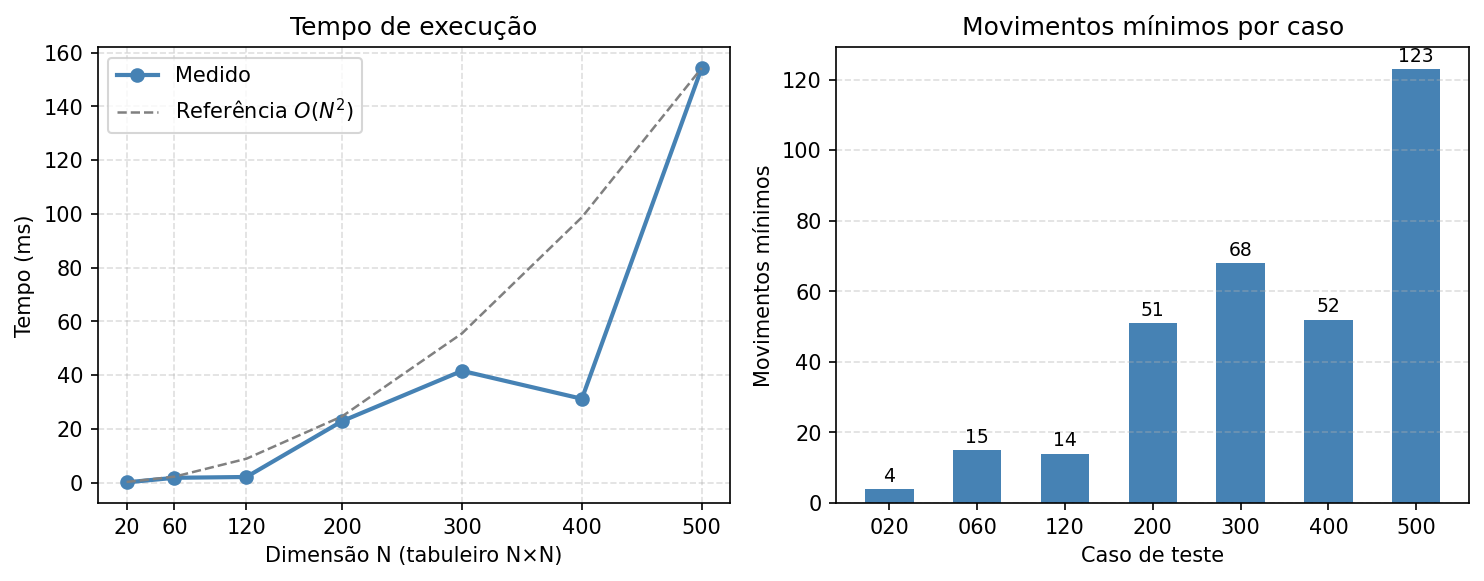
\includegraphics[width=\linewidth]{performance.png}
\caption{À esquerda: tempo de execução em função da dimensão $N$, com curva de
referência $O(N^2)$ escalada pelo ponto final. À direita: número mínimo de movimentos
por caso de teste.}
\end{figure}

\vspace{0.4em}
\renewcommand{\arraystretch}{1.3}
\begin{center}
\small
\begin{tabular}{lcccrr}
\toprule
\textbf{Arquivo} & \textbf{Dimensão} & \textbf{Posição C} & \textbf{Posição S}
                 & \textbf{Mínimo de movimentos} & \textbf{Tempo (ms)} \\
\midrule
020.txt & $20  \times 20$  & (19, 16)   & (7, 14)    & \textbf{4}   & $<$1 \\
060.txt & $60  \times 60$  & (24, 48)   & (49, 6)    & \textbf{15}  & 2    \\
120.txt & $120 \times 120$ & (115, 65)  & (16, 82)   & \textbf{14}  & 2    \\
200.txt & $200 \times 200$ & (109, 91)  & (161, 188) & \textbf{51}  & 23   \\
300.txt & $300 \times 300$ & (103, 136) & (22, 15)   & \textbf{68}  & 42   \\
400.txt & $400 \times 400$ & (242, 164) & (190, 66)  & \textbf{52}  & 31   \\
500.txt & $500 \times 500$ & (347, 282) & (354, 36)  & \textbf{123} & 154  \\
\bottomrule
\end{tabular}

\vspace{0.3em}
{\small Tabela 1: Resultados dos sete casos de teste. Tempos medidos em Python numa
execução representativa; variam conforme a máquina.}
\end{center}

\vspace{0.4em}
Observa-se que o número de movimentos não cresce monotonicamente com o tamanho do
tabuleiro: o caso $120 \times 120$ exige menos movimentos (14) do que o $60 \times 60$
(15), e o $400 \times 400$ (52) menos do que o $200 \times 200$ (51). Isso ocorre
porque a dificuldade depende da posição relativa de \texttt{C} e \texttt{S} e da
distribuição dos obstáculos, que são independentes em cada instância.

O gráfico de tempo confirma o comportamento $O(N^2)$: a curva medida acompanha a
referência quadrática, com o caso $500 \times 500$ (250\,000 células) resolvido em
menos de 200\,ms.

\newpage

\section*{Conclusões}

O problema \emph{O Cavalo Perdido} foi modelado como busca pelo menor caminho em um
grafo não-ponderado sobre um tabuleiro toroidal com obstáculos. A escolha de BFS
mostrou-se adequada e eficiente:

\begin{itemize}[leftmargin=2.2em,itemsep=0.4em]
  \item \textbf{Otimalidade:} BFS garante o menor número de movimentos em grafos
        não-ponderados.
  \item \textbf{Eficiência:} complexidade $O(N^2)$ em tempo e espaço, com todos os
        casos resolvidos em poucos milissegundos.
  \item \textbf{Corretude no tabuleiro toroidal:} a aritmética modular garante que
        os movimentos que cruzam bordas são tratados corretamente.
  \item \textbf{Impossibilidade:} quando não existe caminho, o BFS encerra após
        visitar todos os vértices acessíveis a partir de \texttt{C} e retorna $-1$.
\end{itemize}

Em todos os sete casos de teste o cavalo conseguiu alcançar a saída. O caso mais
simples exigiu 4~movimentos (tabuleiro $20 \times 20$) e o mais complexo
123~movimentos (tabuleiro $500 \times 500$).

Uma possível extensão seria explorar heurísticas admissíveis para A*, o que poderia
reduzir o número de estados explorados em instâncias com solução de muitos passos.
No entanto, dado o desempenho já obtido com BFS puro, tal refinamento não se mostrou
necessário para os casos de teste fornecidos.

\newpage

\section*{Referências}

\begin{enumerate}[label={[\arabic*]},leftmargin=2.4em,itemsep=0.3em]
\item Cormen, T. H.; Leiserson, C. E.; Rivest, R. L.; Stein, C.:
      ``Introduction to Algorithms'', 3rd ed. MIT Press, Cambridge, 2009.
\item Sedgewick, R.; Wayne, K.:
      ``Algorithms'', 4th ed. Addison-Wesley, 2011.
\item Skiena, S. S.:
      ``The Algorithm Design Manual'', 2nd ed. Springer, 2008.
\end{enumerate}

\vspace{1.2em}
\noindent\textbf{Declaração de Uso de Inteligência Artificial:}
Declara-se o uso de Inteligência Artificial Generativa (modelo Claude) como ferramenta
de suporte durante o desenvolvimento deste projeto e a redação deste documento, restrita
a funções de revisão textual, adequação de referências à ABNT e consultas técnicas de
programação. Em conformidade com a Portaria CNPq Nº~2.664/2026, os autores assumem
responsabilidade integral sobre a veracidade, originalidade e validação de todo o
conteúdo e código aqui apresentados.

\end{document}
